\documentclass{article}


\usepackage{arxiv}

\usepackage[utf8]{inputenc} % allow utf-8 input
\usepackage[T1]{fontenc}    % use 8-bit T1 fonts
\usepackage{hyperref}       % hyperlinks
\usepackage{url}            % simple URL typesetting
\usepackage{booktabs}       % professional-quality tables
\usepackage{amsfonts}       % blackboard math symbols
\usepackage{nicefrac}       % compact symbols for 1/2, etc.
\usepackage{microtype}      % microtypography
\usepackage{graphicx}
\usepackage[
backend=biber,
style=nature,
sorting=none
]{biblatex}
\addbibresource{references.bib}
\graphicspath{ {./images/} }


\title{Digital contact tracing in the fight against COVID-19}


\author{
 Hardik Gupta \\
  Harvard University\\
  Cambridge, MA 02138 \\
  \texttt{hardikgupta@g.harvard.edu} \\
  %% examples of more authors
   \And
 William Seaton \\
  Harvard University\\
  Cambridge, MA 02138 \\
  \texttt{wseaton@g.harvard.edu} \\
   \And
 Johannes Kolberg \\
  Harvard University\\
  Cambridge, MA 02138 \\
  \texttt{johanneskolberg@g.harvard.edu} \\  
  \And
 Andres Colubri \\
  Broad Institute of MIT and Harvard\\
  Cambridge, MA 02142 \\
  \texttt{andres@broadinstitute.org} \\
}

\begin{document}
\maketitle
\begin{abstract}
Digital contact tracing has been extensively touted as an effective approach to track and contain the spread of the COVID-19 pandemic and allow safe reopening of social and economic activities in the United States and around the world. This approach uses technology native to mobile smartphones to rapidly identify possible SARS-CoV-2 exposure, contact exposed citizens, and advise targeted self-quarantine measures. However, countries have adopted a variety of different technologies that have collectively been labelled as "contact tracing". Furthermore, there are important design choices involved in the engineering and policy solutions associated to these technologies that impact privacy and civil liberties. In this paper, we explore the efficacy of the different contact tracing programs adopted by national government responses and their associated privacy costs. We also study the impact of digital contact tracing using a simple simulation model. This model allows us to examine population's infection rate as a function of user adoption and compliance, as well as the patterns of epidemic containment under various scenarios of progressive reopening. We find that app penetration of between 40-60\% of the population is necessary to reduce spread of the disease to a level manageable by a major hospital system, in line with previous findings, though this requires adherence to the app’s recommendations of 50-60\% at minimum. When paired with a stay-at-home order, digital contact tracing successfully contains our simulated COVID-19 below manageable levels. We also find that digital contact tracing during staged lifting of activity restrictions could reduce the risk of a second wave of infections, if app penetration and compliance are both roughy over the 60\% threshold. In reality, such ideal metrics of technology adoption are hard to attain, even in countries with a coordinated public health response and higher acceptance by the population of government-mandated interventions.
\end{abstract}

\section{Introduction}

\subsection{Situation Description}

Entering June 2020, the United States has passed 1.75 million COVID-19 cases and represents a third of the world’s cases \cite{Coronavirus_US}. More than 100,000 people have died from the disease despite stay-at-home orders in place for the past eight weeks. Some states have succeeded in efforts to “flatten the curve” by reducing the viral growth rate to an amount manageable by the hospital system, but in others, the growth rate yet increases. Continued efforts are still required to eliminate the pandemic, but these efforts are beginning to cause their own second-order damage. The extended duration of stay-at-home orders has slowed economic activity at the fastest rate since the Global Financial Crisis of 2008 and, by some measures, since the Great Depression of the 1930s. The economy declined by 4.8\% in the first quarter of 2020 with a further drop expected in the second quarter \cite{GDP_FRED}. More than 30 million people in the US have filed for unemployment benefits during the six weeks ending on April 25th 2020, the fastest rate in the nation’s history \cite{Unemployment_US}. The magnitude of these second-order impacts of mitigating the epidemic are causing politicians to begin arguing that the solution cannot be worse than the disease and proposing various plans to re-open the country. Public health experts have stated that any plan to reopen the United States will require tools like sufficient testing capacity and contact tracing, the latter of which is our focus.

Contact tracing is defined by the World Health Organization as the “identification and follow-up of persons who may have come into contact with a person infected.” \cite{ContactTracing_WHO} It allows for an understanding of the magnitude of public health risk from exposure and a targeted method of advising exposed individuals on proper medical precautions, typically focused on self-isolation to prevent further transmission. It helps both in combating the spread of the disease and in our epidemiological understanding of it.

Contact tracing is traditionally a manual process, involving interviewing the patient about their recent travel history, listing each of the people they came into close contact with and a phone number to contact them, and following up with each contact to alert them to their exposure and advise on recommended actions. Privacy concerns exist because each patient is providing the government with a list of their known contacts and detailed records of their whereabouts. In some countries such as Singapore, providing this information is required by law if you have been tested and confirmed ill. Though it would damage containment efforts, the patient does have a choice to not reveal certain travel locations and personal contacts. Additionally, accuracy relies on the memory and truthfulness of the patient and is limited to only their personal acquaintances. If the patient was asymptomatic and within six feet of someone on a public bus, they will not know that person’s contact information in order to follow up and notify them. Each interview can take an hour or more to gather this information and subsequent phone calls depend on the prompt response of exposed individuals. For diseases with high transmission rates, manual contact tracing can be too slow to keep up and provide real containment.

Manual contact tracing is also very expensive. Tom Frieden, former director for the Centers for Disease Control and Prevention, estimates that the United States will need to hire 300,000 contact tracers to contain COVID-19 after re-opening. David Harvey, executive director of the National Coalition of STD Directors, estimates 30,000 new contact tracers from today’s 1,600 but puts the cost of these new hires at \$720 million \cite{ContactTracers_STAT}.  Massachusetts has taken the lead amongst the states by hiring 1,000 new contact tracers and allocating \$44 million towards the initiative. Early evidential costs are large and will put a further strain on spending by the federal government. Fortunately, there are opportunities to significantly reduce both time and cost requirements.

Digital contact tracing is an opportunity to use ubiquitous mobile technology to greatly accelerate the monitoring and alerting of possible exposure incidents. In principle, it eliminates the reliance on faulty human memory and can for enrolled participants eliminate the time taken to disseminate infectious contact alerts through that patient’s network. The perceived potential of this technology to enable a safe lifting of strict social distancing measures lead to a frenzy of activity from individuals and groups around the world to create contact tracing apps for COVID-19 \cite{TechRevTracker, CovidTracking}. As with many digital advances, the benefits of speed and efficiency risk including a loss of individual privacy, with a proportion that depends on the implementation\cite{HealthAndLiberties}. For example, digital contact tracing can require collecting and sharing your detailed location data for as long as 28 days with a government health agency or private company. It becomes simple to identify your personal network and the strength of each connection according to the time spent in physical proximity. If data processing occurs within government IT systems, opportunity for abuse exists should an analyst process the data in ways unrelated to contact tracing. In the United States, data retention laws can be limited and patients may be unaware how long the government will retain this information once the disease has dissipated. The possibility for abuse has privacy advocates in academia and industry leaping to develop solutions that are effective, efficient, and respect individual privacy. In addition to these issues, the use of digital contact tracing also poses questions about equity of access by vulnerable populations\cite{AddressingEquity}.

\subsection{Technology Choices and Design Decisions}
Mobile phones provide two primary methods of digital contact tracing: Global Positioning System (GPS) and Bluetooth. Both come standard with most modern smartphones. GPS provides detailed locations for an individual at hyper-specific time intervals. It is commonly used in consumer applications, so there is a large population of application developers with familiarity in designing GPS-based applications. While location data is detailed, it is most useful for two-dimensional spatial analysis and can provide frequent false positives when applied to digital contact tracing. Analysts struggle to accurately evaluate vertical distances or intermediate barriers and may falsely assume two people were close enough to spread a disease when in fact they were several floors apart. Bluetooth contact tracing relies on signal strength, specifically a calculation called the Received Signal Strength Indication (RSSI), to measure proximity and distance of two devices \cite{BluetoothTech}. This signal is weakened by intervening objects and is thus less likely to create a false positive for people on the other side of a wall or on different floors. It is also a cheaper technology, so for national initiatives that wish to consider users without smartphones it would be more cost-effective to use Bluetooth devices \cite{Trackers}. 

In addition to the choice of underlying technology, developers must consider the manner in which they develop their digital contact tracing applications. Many institutions have made the underlying code open-source and freely available. Several have partnered closely with government institutions during development or subsequently during data collection; the extent of this partnership can impact the public’s perception of the application and its desire to adopt it. Storage centralization is the key decision to make when working closely with a government agency: most implementations require at minimum a central communication server for coordinating the sharing of lists with potential exposure amongst individual phones; the maximum involves the collection and storage of personally identifiable information (PII) in a central server with access provided to a number of different government agencies with varying missions.

Privacy decisions must also be made around the duration for which data is stored. Public health policy recommends 14 days of quarantine before a person can confidently assume they do not have the disease. Since COVID-19 has high asymptomatic transmission rates, 14 days is considered the minimum number of days that location or interaction data must be stored. Our study found a maximum of 28 days of data storage in the MIT “Private Kit: SafePaths” application.

Another design decision involves user consent: is the user able to opt-in to digital contact tracing or are they mandated to download an application? Some governments require application download for infected patients or travelers entering from abroad, but do not make it generally mandatory. Others restrict all forms of travel unless a user has downloaded the application and has a clean bill of health. Some will send police to your home if you are not using the application as designed to communicate your health to the monitoring government agency.

\section{Review of Current Contact Tracing Approaches}

We explore the various alternatives in a series of case studies, starting with a number of US-centric protocol proposals and implementations (Private Kit, TCN, and Apple/Google's API) that would enable interoperability between different contact tracing apps while ensuring privacy of users, and then navigating from those nations with the most pervasive data collection to those with the strictest privacy policies.

\subsection{US Protocols for Digital Contact Tracing}

The United States’ lack of a cohesive federal response has prevented a single approach from taking shape. Instead, a variety of methods have been proposed by academic research groups and private companies like Apple and Google – the largest developers of mobile phone operating systems. We explore the most prominent applications proposed by universities like Stanford, the University of Waterloo, and MIT. Their work has impacted major design choices being made by Apple and Google, who have announced the integration of Bluetooth-based contact tracing into their core platforms.

\subsubsection{MIT’s “Private Kit: SafePaths”}
MIT has been leading the development of the SafePaths application \cite{COVIDSafePaths}. SafePaths stores 28 days of GPS and Bluetooth location history locally on your phone and allows you to share it with the SafePaths community and public health officials if you have tested positive for COVID-19. The project is open-sourced \cite{COVIDSafePathsSource} and built with “privacy-by-design.” The app compares an individual’s location history to anonymized public location data of known infected patients. The comparisons are done locally on the user’s phone and no data is shared unless the user approves it. When a patient tests positive, they will work with a medical professional to review their location data and publish 14 days of travel history to SafePaths’ central repository.

SafePaths has targeted public health officials as a beneficiary with its associated web-tool “SafePlaces”, which maps hot spots of confirmed COVID-19 cases to improve resource allocation prioritizations \cite{COVIDSafePathsFAQ}. They also claim a secondary benefit of GPS mapping for users who can now avoid infection hotspots. Government agents are only able to access anonymized location trails of infected patients, which SafePaths says provides the added benefit of identifying public locations with frequent COVID-19 exposure beyond what Bluetooth alone can provide. SafePaths shares that health officials can manually redact personal locations like home or work but leaves redaction decisions to the government agent in collaboration with the user. This leaves the concern that if not redacted, someone could re-identify the individual by comparing their frequently visited locations to identify their home, workplace or neighborhood \cite{MobilityTraces}. 

SafePaths’ rejection of Bluetooth as the primary location technology appears shallow. They quote that “there are some widespread third-party apps that have hundreds, or even sometimes billions, of installations” that can “start listening to all these Bluetooth beacons that are being emitted by these phones and can easily create the identifiable trajectories.” \cite{Transparency} While there have been some studies that use “sniffing” algorithms to maliciously identify a user’s location \cite{VulnerableToTracking}, these have typically been issues of neglect resulting in the lack of random ID generation or encryption – both common security protocols.

SafePaths has proposed an effective and decentralized method of digital contact tracing yet should ultimately be evaluated on the basis of the necessity of specific location history in containing the virus. The anonymized heat map of infected patients can help public health officials and users target areas for containment or avoidance, but it is not clear this targeting needs to be so granular. Public resource allocation typically happens at the hospital or zip code level, information that can be gathered manually from COVID-19 patients. Contact tracing happens at the level of individual interactions, something managed equivalently well with Bluetooth-only methods. The app designers acknowledge that location data such as commuting times will need to be manually removed from the public repository as unimportant for public health, yet this will be what the majority of GPS data will provide above someone manually listing their most frequent locations. The utility benefits from collecting and utilizing GPS data do not appear to outweigh the privacy concerns.

\subsubsection{Stanford and Waterloo’s “TCN Protocol”}
One of the most secure proposals for digital contact tracing has come from researchers at Stanford University and the University of Waterloo. Their app “Covid Watch”\cite{CovidWatch} uses a decentralized, randomly generated token list to maintain a local history of interactions as measured by the strength and duration of Bluetooth signal. When a patient tests positive for COVID-19, their private local list of interaction tokens are sent to a central server of “infected tokens” with no PII associated. The central server publishes to all participating mobile phones the full list of “infected tokens” so that local processing can compare “infected tokens” against a phone’s list of interaction tokens to confirm if that particular user has had any close interactions with an infected person. At no point does the central repository or any other user receive PII that could be used to identify who is infected or who interacts with whom. This open-source design is called the “Temporary Contact Number (TCN) Protocol.” \cite{TCNProtocol}

In addition to recording no PII, the TCN protocol randomly generates a new contact event number every few minutes so each phone has no unique identifiers that could be used for re-identification. This helps to prevent the prominent method of Bluetooth hacking where a physically proximate malicious actor could track a persistent Bluetooth ID to identify the broadcaster’s location.

This method of background Bluetooth exchange is handicapped by policies in place with the two primary mobile operating system developers, Apple and Google. Apple’s iOS does not allow persistent Bluetooth broadcasting in the background as a privacy precaution, while Google’s Android does with user permission – but has unfixed bugs where repeat connections between multiple devices can cause Bluetooth to lock up.

The TCN Protocol is the approach to digital contact tracing that appears both fully effective for public health measures and respectful of user privacy. Still, Stanford computer scientist and team lead Cristina White acknowledges that the protocol has seen slower adoption by public health officials because of its lack of GPS data. “Public health agencies really don’t want to do the kind of thing that we’re proposing because they do want more data. But I think we’re providing what the public might want.” \cite{CryptoProtection}

\subsubsection{Apple and Google's COVID-10 Exposure Notification API}
The two largest mobile phone operating system developers, Apple and Google, have sole approval rights on the design of applications allowed in their respective App Stores, and therefore control the associated probability of success for any nascent method of digital contact tracing. It is therefore encouraging to see that the decisions they have made to support digital contact tracing have been impacted by privacy advocates. The companies announced a joint partnership to build into their core platforms a form of Bluetooth-based contact tracing \cite{AppleGoogle}. In May, the companies will release a cross-platform API to enable apps built for their audiences to communicate with one another, preventing a situation where users are only able to connect with others using the same phone type. In the coming months, both companies will build opt-in Bluetooth-based contact tracing directly into their core platform, eliminating the need to download one of an increasing number of applications. There are several reasons to be optimistic about this. First, the companies have sought input from and listened to public health experts and privacy advocates in choosing how best to assist in the fight against COVID-19. Second, the companies elected to make this service opt-in. Third, the companies have a combined installation base of over 3 billion smartphones worldwide. The immediate international impact of this privacy-preserving technology installed by default can pay major dividends in the fight against COVID-19 and future disease outbreaks.

\subsection{Policy Formation Around the World}

Many countries have made digital contact tracing a prominent tactic in containing COVID-19 \cite{ContactTracingWorld}. Different national cultures and the relationship between citizens and their government has led to different choices in technology, centralization, and the extent to which compliance is mandatory. The countries that best succeeded in containing the virus all laud digital contact tracing as necessary in their efforts, but the underlying approach has differed dramatically. 

\subsubsection{China}
China implemented the strictest response to the novel coronavirus using pervasive data collection, enforcing mandatory data sharing, location tracking, and restricting the movement of its citizens according to a health score. The country restricted travel by instituting a color-coded rating system delivered via a QR code across several major app ecosystems \cite{ChinaColorCodes}. Local governments defined the rating algorithm logic and colors were used at public checkpoints to determine whether police would permit an individual to pass and leave their neighborhood. Green codes permitted unrestricted movement, yellow codes required seven days of quarantine and red codes required fourteen. Users downloaded the apps from China’s major platforms Alibaba, Tencent and Baidu, and were required to share information at sign-up such as their name, national identity card number, phone number, home address, potential symptoms and travel history. Continuous data collection occurred as users were required to enter their temperature each day to maintain their health status.

\subsubsection{South Korea}
South Korea has been looked upon as an exemplar response to COVID-19 from a democracy, but the details of their data use have cause for concern when viewed from a privacy perspective. The government emphasized transparency in metrics and diagnosis, localization of alerting, and detailed contact tracing. Once a person has a positive COVID-19 test, the city or regional government will push a public notification to all local residents including personal information on the patient such as last name, sex, birth year, residential district, profession, hospital and travel history. Additionally, contact tracers integrated closed-circuit television (CCTV) and credit card data to gain the fullest picture of a patient’s recent travel. \cite{KoreaPersonalData}

The government has a strong legal basis for data transparency around infectious diseases coming from frameworks made in response to the 2015 outbreak of Middle East Respiratory Syndrome (MERS). At the time, they refused to publish which hospitals were treating MERS patients until a citizen developer made a map of crowd-sourced reports and anonymous tips from hospital staff. The publication of this information combined with public backlash against the secrecy forced the government to release greater detail. This change was codified in 2015-2016 with notable amendments to South Korea’s Infectious Disease Control and Prevention Act (IDCPA)\cite{KoreaLawUse}. The first relevant amendment was to Article 76-2(2) and permitted the Minister of Health and Welfare to request from the National Police Agency “location information of patients with an infectious disease and persons likely to be infected by an infectious disease” and forced any “location information provider and the telecommunications business operator” to comply with the police request. The second was to Article 6(2) and stated that “each citizen shall have the right to know information on the situation of the outbreak” and “local governments shall promptly disclose the relevant information.” \cite{KoreaIDAct}

Studies find that South Koreans are supportive of data transparency and collection, favoring the right to know over the right to privacy during a pandemic\cite{KoreaCaseDetails}. Still, the transparency has led to a hesitation to proactively get tested, according to Choi Young-ae, the chair of South Korea’s Human Rights Commission (HRC) \cite{QuarantineFreeTech}. While the government tried to localize its alerts, citizen developers have again built applications that gather all alerts and publicize them in a central location. Applications like Citizen Map and Citizen 100m have been downloaded by more than a million people. In response to the HRC, South Korea’s CDC issued limited updated guidance on March 14th that reduced the time duration of released history according to the severity of symptoms and stated “personally identifiable information should be excluded” but re-stated its support for releasing “spatial and temporal information such as buildings and place names.” \cite{KCDCMarchUpdate} This appears to have been enough information to continue to support public shaming campaigns being pursued by some internet users against those patients who had been re-identified.

\subsubsection{Poland}
Poland was one of the first European countries to launch a smartphone application for digital contact tracing, mandating its download for infected patients and citizens returning from abroad. At sign-up, users can see a number of personal details auto-completed from existing government databases. The application uses GPS location data to ensure the user has remained indoors. It validates a person has not left their phone behind by requiring the user to submit a self-photo within 20 minutes of receiving a random check-in text message several times per day. The application shares data with a number of government agencies and the police, who can levy fines of up to 6,550 euros for breaking quarantine\cite{PolandApp}. 

Efficacy questions abound. The application was launched after three days of development and reportedly came off a simple template application design and crashes frequently. Exceptions exist for those who cite poor Internet connectivity or no smartphone. The app frequently freezes or fails to send the required self-photo, causing stress when the time permitted and the time displayed disagree. One user reported that the police cleared him to leave quarantine while the app continued to request selfies. Poland is the only example we found that required some form of facial recognition to validate location. It is also an interesting example where implementation quality raises further privacy concerns. Even if the government guaranteed no data storage of submitted selfies, the frequency and variety of app failures implies vulnerabilities and design gaps in the app itself as well as in storage or transfers of data.

\subsubsection{Taiwan}
The country of Taiwan has received much acclaim for its handling of COVID-19. It combined rapid response, policy flexibility, and technological innovation to contain the virus and reported no new cases for the first time on April 14th, though new spikes have occurred since. It reduced new cases to zero for the first time within 36 days and has reported just 441 total confirmed COVID-19 cases as of May 28th, 2020 \cite{TaiwanNoCases}.

Taiwan does not use GPS to track a person’s location, but instead relies on the relative signal strength of a single cell reception tower to understand if someone under quarantine is remaining at home \cite{TaiwanDigitalFence}. If the signal strength changes dramatically, drops off, or if the cellphone begins pinging a different tower, it can be assumed that the person has moved from their assigned quarantine home. When this happens, first responders are dispatched to the user’s home but only receive the person’s name, phone number and address to minimize privacy infringement to just what is necessary for law enforcement actions. The country cites a 1\% false alarm rate\cite{TaiwanTrackingSystem} and is partnering directly with telecom service providers to reduce errors further.

The mandatory electronic fence is being applied to infected individuals and travelers entering from abroad, impacting both citizens and non-citizens. The police will call the phone twice a day to ensure the individual has not left their phone at home. There have been anecdotal news reports that zero phone movement will also trigger a notification to the police as another method to identify if the person has left their phone at home. Breaking quarantine results in a fine of 1,000,000 NTD (~\$33,000 USD)\cite{TaiwanDigitalFence2}.

Mandatory quarantine for patients and travelers is a strict response that most Western governments have avoided to date. This question strikes at the core of how much power is given to the government during war or pandemics. Under what circumstances should the government have the power to restrict the movement of its citizens? The answer varies by each country’s cultural relationship with their government and liberal philosophy. The Taiwanese government deserves credit for restricting location tracking to those reasonably impacted by COVID-19 – instead of instituting mass surveillance, as China did – and for finding a functional alternative to blanket GPS tracking through the creative use of cell phone tower pings.

\subsubsection{Singapore}
Singapore had the first successful national implementation of Bluetooth-based digital contact tracing and became a model for other nations. The app TraceTogether was developed by Singapore’s Ministry of Health and Government Technology Agency (GovTech) and has seen adoption by 25\% of the city-state’s citizens, over 1.5 million people\cite{TraceTogether}. Adoption was slower than desired, reaching 12\% of the population on April 1 and 20\% by April 30th\cite{USLearn}. Singapore’s prime minister Lee Hsien Loong mentioned TraceTogether in an April 21st remark to the nation, imploring more citizens to download the application\cite{SingaporeAprilSituation}. 

TraceTogether collects a single piece of personal information – your phone number – so that health officials can contact you faster in case of suspected exposure. TraceTogether also collects anonymized app analytics data to improve performance, though they only list device model and app version as examples on their website\cite{TraceTogetherData}. Interaction lists are stored for 21 days before deletion and require consent given to the Ministry of Health before the data is publicized. They list a support website you can email to revoke your data storage consent at any time. However, Singapore does have a legal requirement that any person who tests positive and is contacted by the Ministry of Health must help the department in mapping their activity and movements. TraceTogether notifies users of this legal requirement on their website in the FAQ section and says it applies to location timelines and logs in physical or digital form, including presumably what the application collects\cite{TraceTogetherConsent}.

\subsubsection{Australia}
Australia is a notable example for discussion because of the rapid pace of application adoption by a Western democracy. The country’s app Covidsafe requests the user’s age range, postcode, phone number and name, though you can provide a pseudonym\cite{Covidsafe}. The information is centrally stored on a government server and the app uses Bluetooth to record close interactions, which are stored locally on phone for 21 days. If the user tests positive for COVID-19, they can elect to share their interactions from the past 14 days with the government. The government has been explicit that police will not have access to government-stored data and this requirement will be backed up by legislation introduced to the Australian parliament. The Australian app is derived from the source code for Singapore’s app, with one change that allows iPhone users to lock their phone with the app open and still have it running.

The prime minister has vocally said that the app relies on consent, is not mandatory and has spun up a public awareness campaign to encourage sign-ups. He has also stated it will be a criminal offence to refuse service or venue access to any Australian citizen who chooses not to use the app, a strong statement in defense of consent. The Australian health minister has said the government was targeting 40\% adoption. In the first 24 hours after launch, over two million Australian citizens downloaded the application, around 10\% of the population and 25\% of the adoption goal\cite{CovidsafeTakeup}. That is the largest non-mandatory application use rate in the West and a testament to the trust citizens will place in their government when they hold privacy and security foremost in the design and communication of technology initiatives.

While adoption was encouraging, the efficacy of the application has since been challenged. Reports indicate that only a few users have been contacted as potentially exposed using Covidsafe's data. The primary challenges have been that the app only works if open on a user's phone, that not all citizens have access to a smartphone and that adoption rates quickly dropped off as the virus was contained and people became less concerned. These remain common concerns to any digital contact tracing solution proposed.

\subsubsection{Germany}
Germany is pursuing a decentralized Bluetooth-based approach but has arrived at this solution only after strong continental debate\cite{PEPPPTvsDP3T}. Its initial plan was to follow the Pan-European Privacy-Preserving Proximity Tracing (PEPP-PT) Bluetooth-based design launched on April 1st\cite{PEPPPTdocs}. The pan-European research team gained momentum early and had 10 countries committed to launching its protocol, including Switzerland and Spain, before a major privacy debate began in Europe on the extent of centralization of data necessary. An opposing framework called Decentralized Privacy-Preserving Proximity Tracing (DP-3T) functions similarly but only uses a central server for communication of the interaction lists of confirmed cases and processes all token generation and list comparisons on each user’s phone\cite{DP3Tdocs}. DP-3T is similar to the TCN Protocol announced by Stanford and Waterloo in North America. 

Legally, DP-3T argues that PEPP-PT fails to follow the General Data Protection Regulation (GDPR) principle for data minimization. Over 300 European academics signed a letter stating that centralization was unnecessary and further that GPS alternatives lacked sufficient accuracy\cite{ContactTracingStatement}. PEPP-PT researchers did themselves no favor by failing to act transparently during development. They failed to publish code or protocols for review, failed to answer questions related to decentralization at press conferences and removed mentions to alternative frameworks from its documentation as those frameworks gained momentum. Their attitude during debate led to some calling them a “trojan horse” for mass government surveillance\cite{StandardsFight}. While the spirited debate and specificity of privacy advocates is commendable, the decision between frameworks appears to have rested ultimately with Apple and Google. As the platform developers, their support for the DP-3T method and refusal to change platform rules to allow background Bluetooth tracking and transmission to an external server forced Germany’s choice. As a result, following a full vote by the European Parliament, Germany and Europe are officially pursuing the most stringent privacy-preserving digital contact tracing option\cite{EUCOVIDapps}. 

\section{Simulating Impact of Digital Contact Tracing}

Our qualitative study of the various implementations pursued by national governments or designed by academic institutions suggests that Bluetooth-based contact tracing solutions are at least as effective as GPS-based solutions while preserving the privacy of the user to a much greater extent. There is also a strong argument that Bluetooth solutions are more accurate, as their signal is impacted by physical barriers and vertical space, eliminating common false positives from GPS. European and US researchers have argued the privacy merits of various approaches and swayed expert opinion towards the decentralized implementation of Bluetooth interactions. While US’ relative lack of data protection laws has allowed for early momentum of GPS apps like MIT’s SafePaths, the announcement by Apple and Google that they will be implementing an opt-in Bluetooth digital contact tracing API will enable an installed user base so large that it cannot be ignored by public health officials. This decision solidly shifts digital contact tracing towards the most privacy preserving option as the default.

With the selection of this technology, the next concern for policymakers should be the adoption rate necessary for containment and disease management. Specifically, what is the percentage of the population that must activate digital contact tracing such that the method outpaces the virus’ transmission rate? Recent studies using compartmental epidemic models have suggested that contact tracing apps requires a relatively high adoption among the population to be effective \cite{Ferrettieabb6936}. We revisit this question using an alternative agent-based modeling (ABM) approach \cite{ABMOverview} where we explicitly represent susceptible and infectious individuals as they move around between their households and public spaces in the city.

Our epidemic ABM simulation allows us to represent migration probabilities between private and public spaces and the associated infection rate within each. Since we do not compute all possible pairwise interactions between individuals, but we rather have exposure events mediated by the common visited spaces, the runtime of the algorithm is linear on the population size instead of quadratic, which would make it possible to simulate much larger populations. We apply varying rates of application adoption and compliance rates in a grid search to output single-day maximum population-level infection rates, and finally define staged scenarios of lifting of stage-at-home orders where movement of individuals out of their households increase progressively from strict stage-at-home to near-normal activity levels.

\subsection{Infection Rate as Function of App's Adoption}

In order to successfully manage COVID-19, the US healthcare system must have sufficient capacity to handle the maximum single day caseload. By having our simulation find that maximum, we can determine if the combination of penetration and compliance will be sufficient.

\begin{figure} % picture
  \centering
  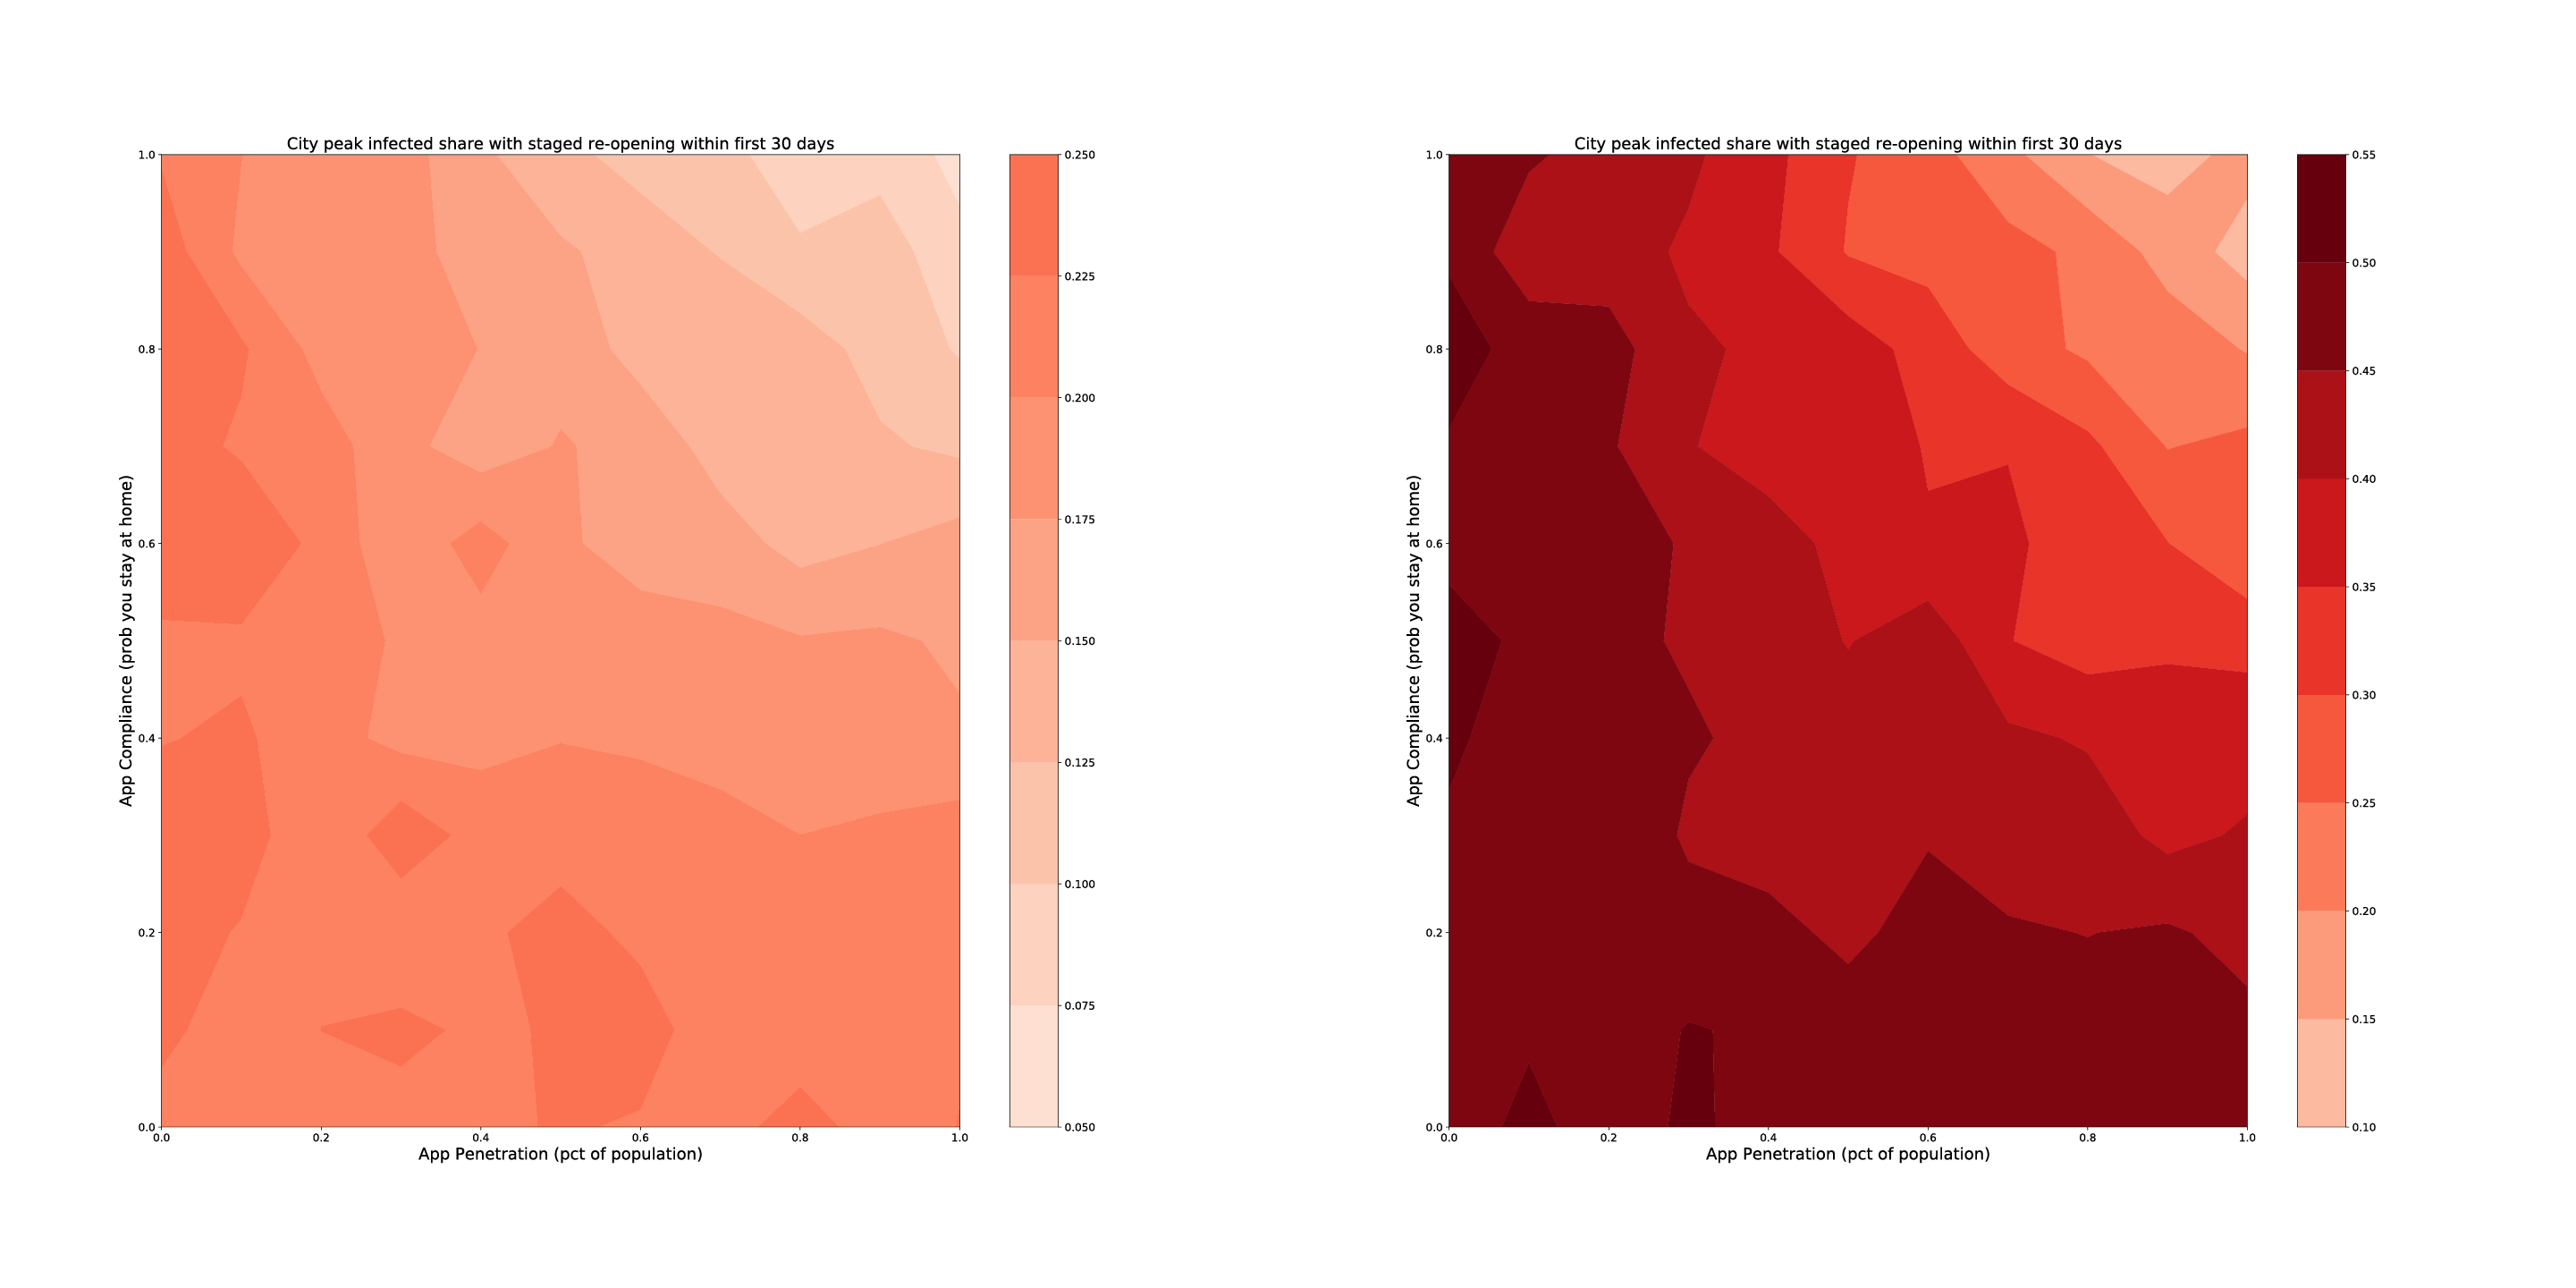
\includegraphics[scale=0.15]{Figure-1.png}
  \caption{ Infection Rates with Stay-At-Home orders (left) and Unrestricted Movement (right)}
  \label{fig:fig1}
\end{figure}

We baseline our target population infection rate using hospital capacity in New York City. The CDC estimates a hospitalization rate among COVID-19 patients of 4.6 per 100,000 patients\cite{PatientCharCDC}. Bloomberg calculates an existing NYC hospital bed capacity of 23,000, with another 18,333 added in recent months using emergency measures\cite{HospitalBedsNYC}. Hospital capacity planners target 85\% average occupancy\cite{HowManyBeds}  while New York City reported in 2018 utilization rates of 79.7\% and 89.7\% depending on the facility type\cite{BedUtilizationReport}. Assuming the low end of utilization, even with the emergency beds, New York City would have just 8,390 free beds for COVID-19 patients. At those rates, New York City with a 2018 population of 8.4 million would require an infected population rate less than 21\% for the hospital system to manage the patient load. To see if that target infection rate was possible, we tested the efficacy of adoption and compliance rates in multiple scenarios representing varying city densities and policy decisions.

First, we simulated epidemic transmission through a city under stay-at-home orders compared against a city with unrestricted mobility. We set probability of leaving one’s private residence at 35\% under stay-at-home orders, as this is the mobility rate Google quotes for France, a Western country that implemented mandatory stay-at-home and so can be assumed to have similar city design as an US city and high stay-at-home compliance\cite{MobilityReportFrance}. We set unrestricted mobility probability at 95\%, applying some discount from 100\% for those with limited ability to leave, such as the sick or elderly.

Our results show that stay-at-home orders remain one of the most effective means of containing COVID-19 transmission (Figure \ref{fig:fig1}). A low probability of leaving your home reduces the maximum single-day infection rate significantly at every parameter test and nearly all levels would be manageable by the health care system. High infection only occurs in the corners where compliance or app penetration is very low. With unrestricted movement, app penetration needs to be greater than 70\% and compliance above 60\% to hit the requisite level.

Second, we wanted to compare application impact in various cities with differing private-to-public ratios and densities. We selected New York City (New York), Austin (Texas) and Omaha (Nebraska) as our three cities representing dense cities with high public-to-private building ratios, sprawling cities with low ratios and an averagely dense US city, respectively. We took the number of households from the United States Census Bureau. To peg our selection of “public spaces” to a shared and easily confirmable statistic, we identified the number of National Historic Landmarks present in each city. While these are not necessarily highly frequented locations, they provide an effective proxy for the public-to-private ratio we were concerned with modeling.

\begin{figure} % picture
  \centering
  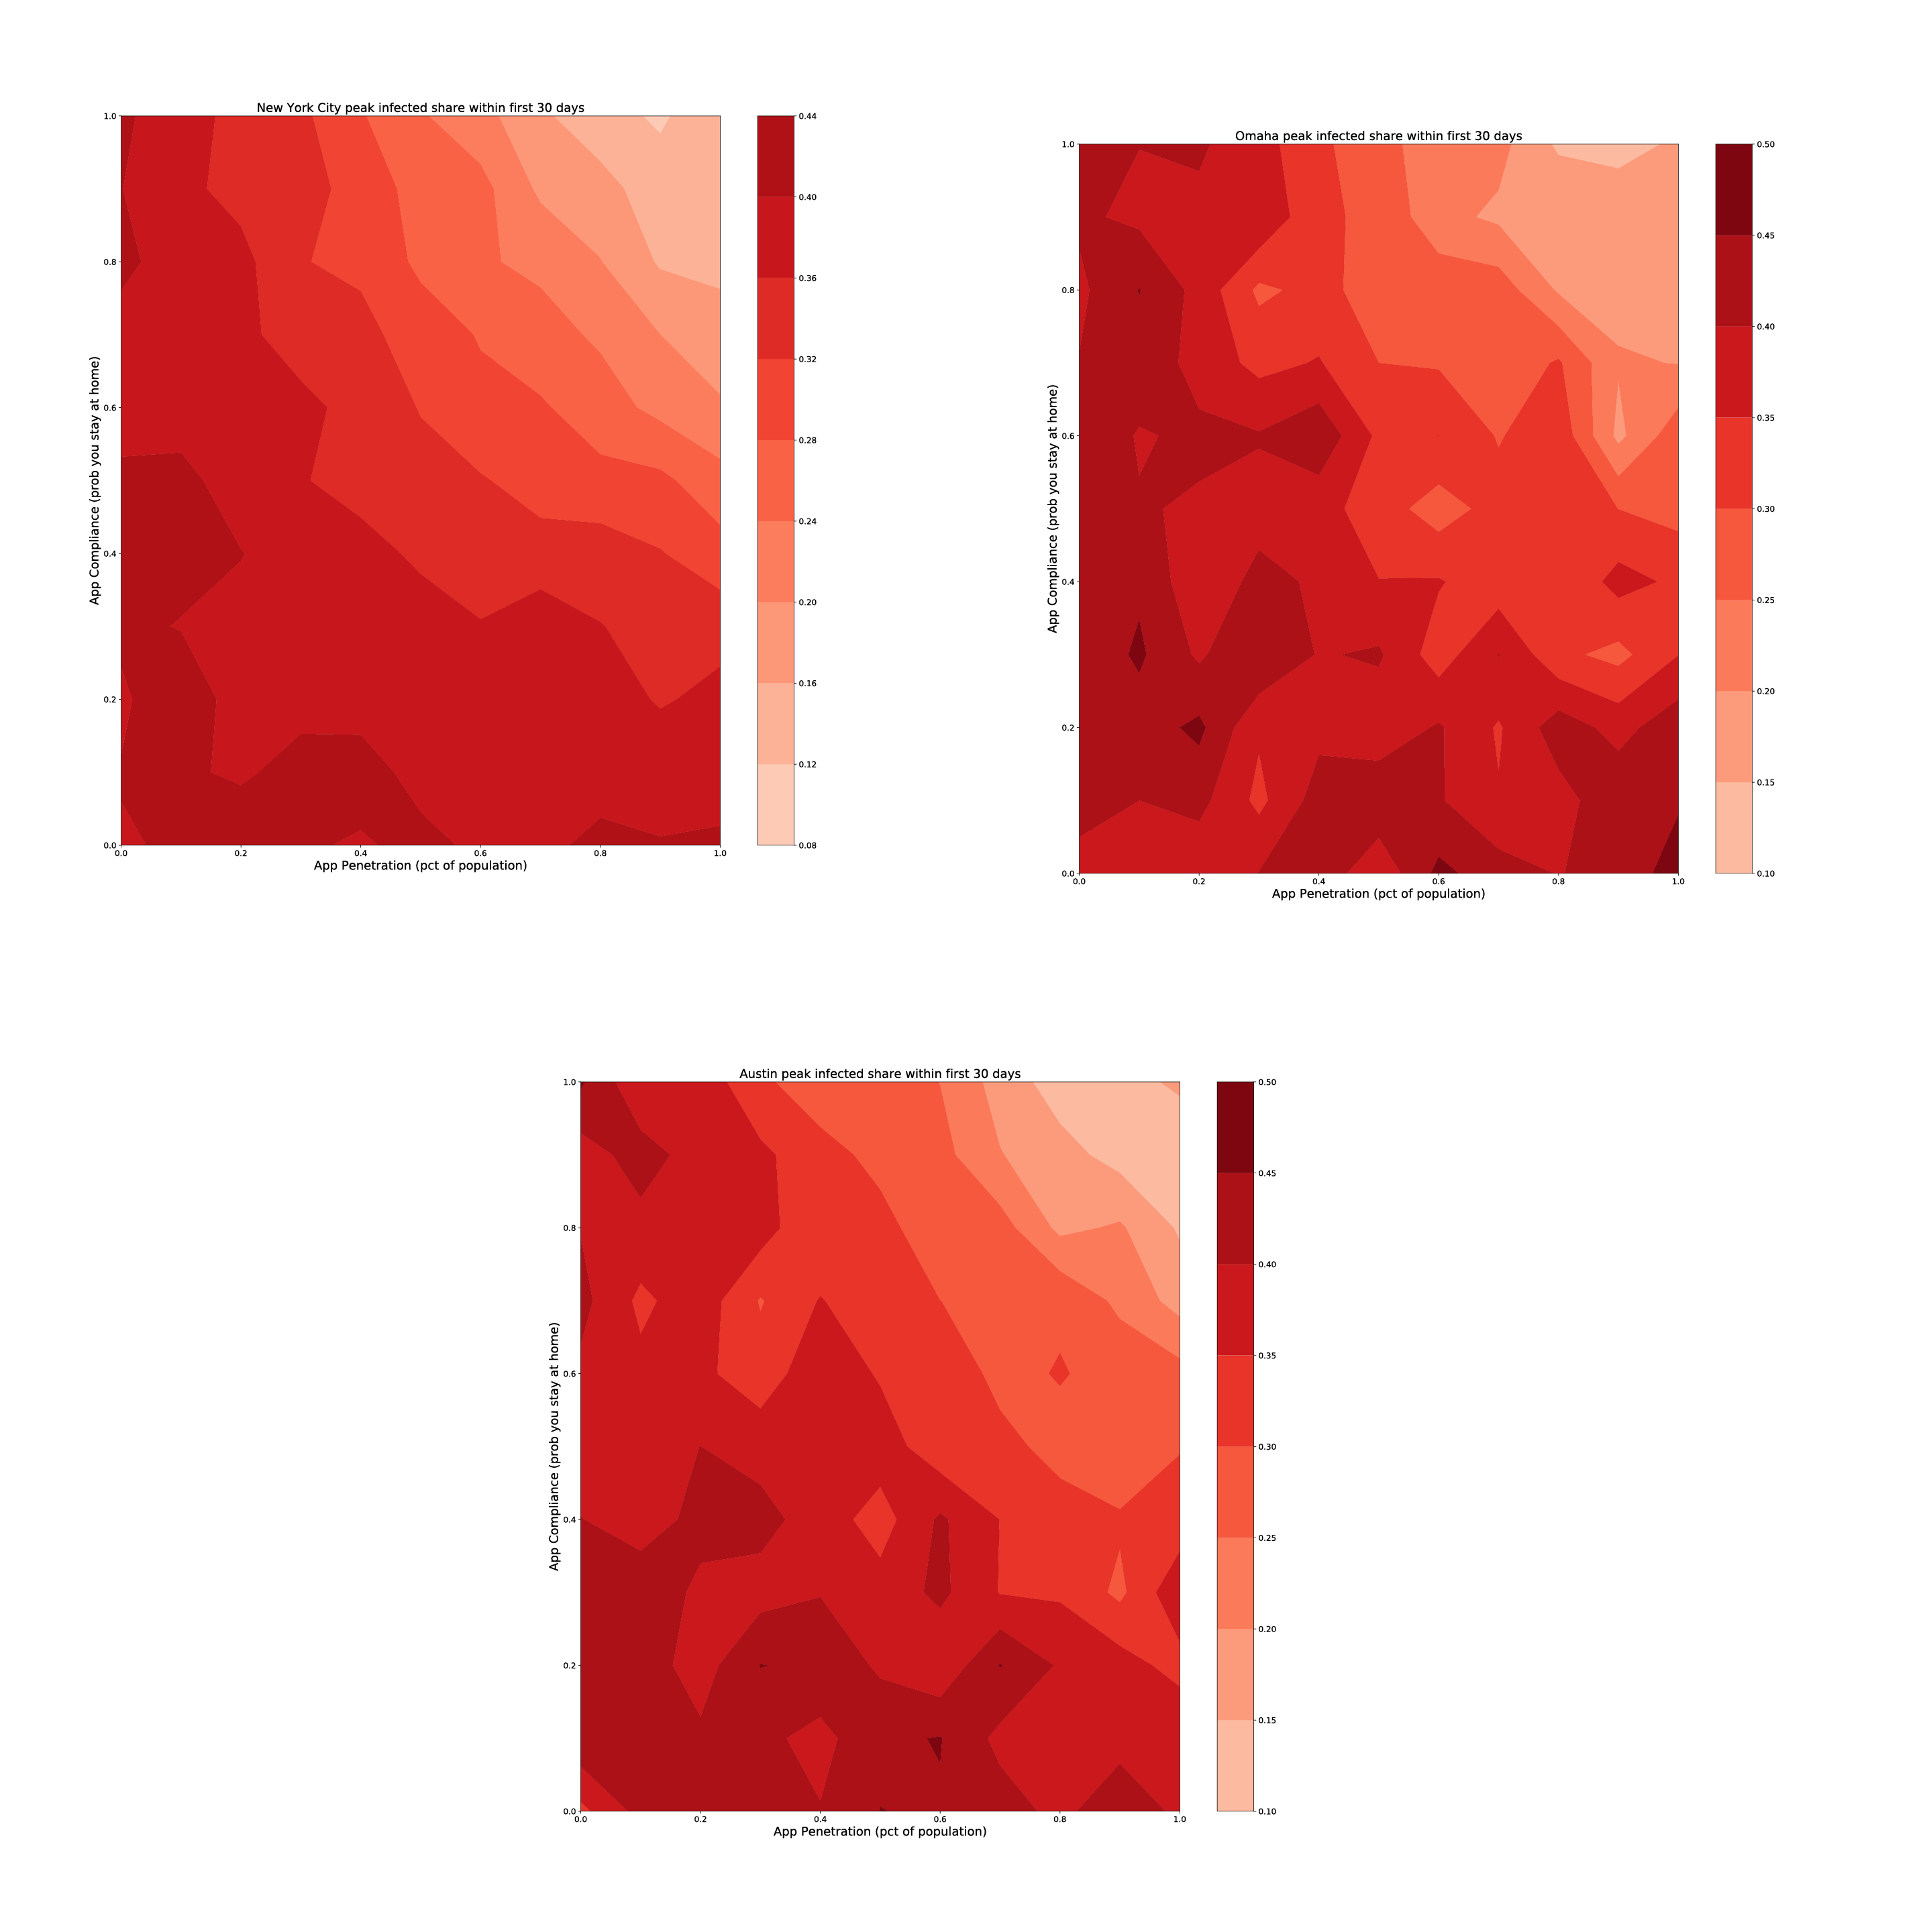
\includegraphics[scale=0.15]{Figure-2.png}
  \caption{Infection Rates in cities like New York (top left), Omaha (top right) and Austin (bottom)}
  \label{fig:fig2}
\end{figure}

In a dense city like New York, with a high public-to-private space ratio, app penetration needs to be around 50\% with compliance at least 60\% to maintain an infected population rate near 20\%. Omaha, a more average US city, would require higher app penetration near 70\% but compliance can be lower at 50\%. Austin, a more sprawling city comparatively, could make do with 40\% penetration but still requires 60\% compliance.

\begin{figure} % picture
  \centering
  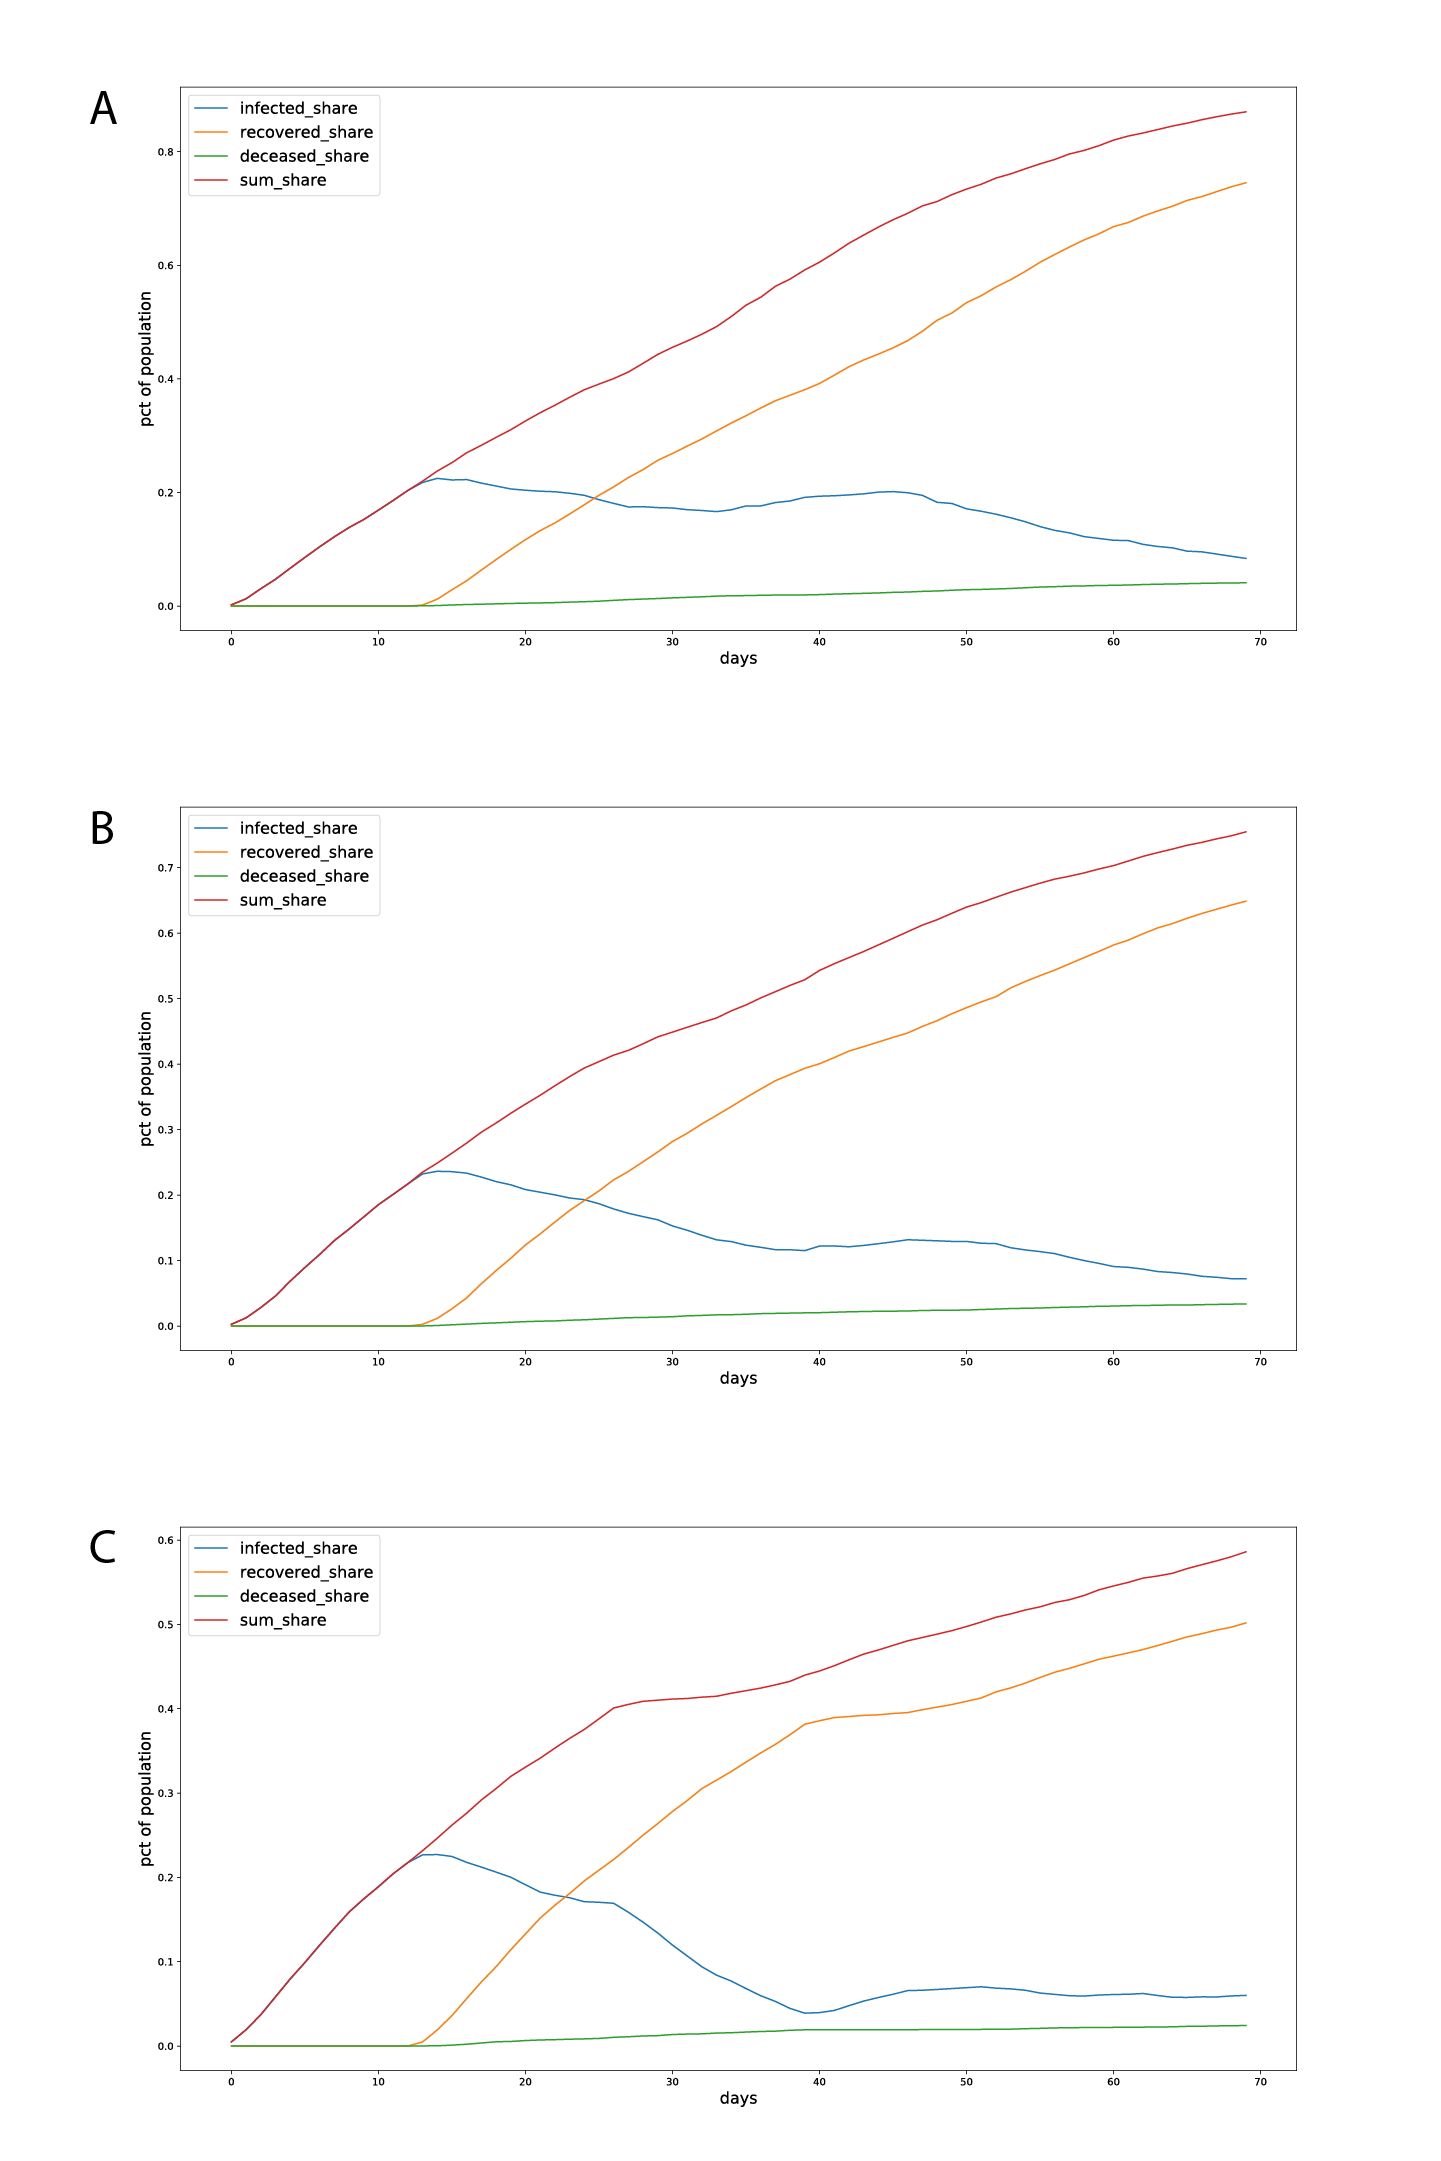
\includegraphics[scale=0.25]{Figure-3.png}
  \caption{Infection Rates in a city like Boston over the course of a 70-day period re-opening. In panel A, the re-opening is carried out without contact tracing, in B, the reopening is aided with digital contact tracing at a penetration rate of 60\% and compliance rate of 75\%, and in C, the app's penetration and compliance are 100\%.}
  \label{fig:fig3}
\end{figure}

\subsection{Re-opening simulations}

Most states in the US have already began carrying out reopening plans \cite{ReopeningUS}. In the case of Massachusetts, this plan involves a four-phase approach to re-open the state after the stay-at-home period that only allowed essential business and services\cite{ReopeningMass}: phase 1 (start) with limited industries resume operations with severe restrictions; phase 2 (cautious), additional industries resume operations with restrictions and capacity limitations; phase 3 (vigilant), additional industries resume operations with guidance; and phase 4 (new normal),  when development of vaccines and/or treatments enable resumption of "new normal". The roll out of this plan began on May 18, with each  phase lasting a minimum of three weeks before proceeding to the next. These phases are subdivided into distinct stages, for example, phase 1 contemplates opening of essential business, manufacturing and construction on May 18, lab space, limited personal services (hair, pet grooming, car washes), and retail (only remote fulfillment and curbside pick-up) on May 25, and office space on June 1. 

Using this plan as a guideline, we simulate a three-week reopening scenario following an initial 27-days period of strict stay-at-home restrictions, with each week increasing mobility by 10\%. Within this scenario, we run simulations with various rates of app penetration and alert compliance, as described earlier, ranging from 0 to 100\%. In order to represent a Boston-like city, we used a ratio of 3,000 households to 10 publicly-visited spaces (grocery stores, retail stores, office buildings, etc.), using published reports \cite{BostonNumbers, BostonMarkets}. The results are shown in figure \ref{fig:fig3}. A re-opening scenario without any contact tracing exhibits a second peak of cases once mobility restrictions are lifted, almost as significant as the initial wave. However, this peak is significantly reduced if the contact tracing app is adopted by at least 60\% of the population, and quarantine alerts are followed by at least 75\% of the users of the app. In an ideal scenario where adoption and compliance are perfect, the number of cases after re-opening remain under 10\% of the total population. 

\section{Discussion}
Pandemics introduce threats to privacy as the tracking of citizens is core to the public health response to any outbreak. The proliferation of digital technology like smartphones has made the potential for tracking easier, but without clear design and policy choices, this tracking takes away privacy rights of a country’s citizens and risks scope creep once the pandemic is contained. The argument to keep these powers in case a new pandemic appears at any time is a seductive one. Fortunately, in the response to COVID-19, privacy advocates in the United States and Europe have risen to the challenge and defined systems that accomplish public health goals while respecting user privacy. Their impact can be seen in the decisions by Apple and Google to make the strictest Bluetooth-based privacy design the default option for digital contact tracing in their underlying mobile systems.

Our quantitative modeling study found that when travel is unrestricted fairly high rates of app penetration and compliance will be required (minimums of 40-60\% and 50-60\% respectively) to maintain a sufficient patient load for a hospital system. Stay-at-home orders and social distancing help dramatically in maintaining lower enough infection rates. Similar levels of app adoption are needed to avoid a second wave of infections after lifting of stay-at-home restrictions. To hit these high numbers, policymakers should follow the example of countries like Australia and Singapore and emphasize that strong privacy restraints are built into any application to encourage download and compliance. Digital contact tracing can become an incredible example where strict user privacy was maintained simultaneously as a major leap in technological innovation and capability was made to fight the deadly COVID-19 pandemic. 

\printbibliography

\end{document}
